\documentclass{beamer}

\usepackage[utf8]{inputenc}
\usepackage[spanish, es-noshorthands]{babel}
\usepackage{amsmath}
\usepackage{amssymb}
\usepackage{graphicx}
\usepackage{xcolor}
\usepackage{tikz}
\usetikzlibrary{automata, positioning, arrows.meta, decorations.pathreplacing}
\usepackage{forest}

\usetheme{Madrid}

% --- Énfasis: negrita + subrayado + color (regla 7 del CLAUDE.md) ---
\newcommand{\destacar}[1]{\textbf{\underline{\textcolor{red!80!black}{#1}}}}
\newcommand{\azul}[1]{\textbf{\textcolor{blue!70!black}{#1}}}

% --- Diapositiva-mapa recurrente (estilo Raudel) ---
% \bloquemapa{<activo>}{<este>}{<titulo>}{<cuerpo>}
% activo = 0 resalta todos (diapositiva de estructura inicial)
\newcommand{\bloquemapa}[4]{%
  \ifnum#1=#2
    \setbeamercolor{block title}{fg=white, bg=structure}\setbeamercolor{block body}{bg=structure!20}%
  \else\ifnum#1=0
    \setbeamercolor{block title}{fg=white, bg=structure}\setbeamercolor{block body}{bg=structure!20}%
  \else
    \setbeamercolor{block title}{fg=white, bg=gray!50}\setbeamercolor{block body}{bg=gray!12}%
  \fi\fi
  \begin{block}{#3}#4\end{block}%
}
% \mapa{<indice activo: 0 = todos, 1..5>}
\newcommand{\mapaitemize}[1]{%
  \begin{itemize}\setlength{\itemsep}{0pt}\setlength{\topsep}{0pt}\setlength{\parskip}{0pt}#1\end{itemize}}
\newcommand{\mapa}[1]{%
  \begin{frame}{Estructura de la presentación}
  \scriptsize
  \setlength{\parskip}{0pt}
    \bloquemapa{#1}{1}{Preliminares}{%
      \mapaitemize{\item Teoría de lenguajes \item Definición de SAT \item Autómata booleano}}
    \vspace{-3pt}
    \bloquemapa{#1}{2}{Gramáticas de concatenación de rango}{%
      \mapaitemize{\item Nociones básicas \item Ejemplo de reconocimiento \item Por qué las RCG}}
    \vspace{-3pt}
    \bloquemapa{#1}{3}{Resolver el SAT por enumeración}{%
      \mapaitemize{\item Algoritmo por enumeración \item Gramática de consistencia}}
    \vspace{-3pt}
    \bloquemapa{#1}{4}{Construir la gramática producto}{%
      \mapaitemize{\item Predicados indexados \item Misma variable, mismo rango \item Ejemplo de reconocimiento \item Correctitud y tamaño}}
  \end{frame}%
}

% --- Información del título ---
\title[SAT y el vacío de la intersección RCG--regular]
{El SAT y el vacío de la intersección de una gramática de concatenación de rango con un lenguaje regular finito}
\author{Luis Alejandro Arteaga Morales}
\institute[MATCOM]{Facultad de Matemática y Computación \\ Universidad de La Habana}
\date{2026}
\newcommand{\tutores}{MSc. Fernando Raúl Rodríguez Flores \\ Lic. Raudel Alejandro Gómez Molina}

\begin{document}

% ===================== APERTURA =====================

% --- 1. Portada ---
\begin{frame}
  \titlepage
  \begin{center}
    Tutores: \tutores
  \end{center}
\end{frame}

% ===================== INTRODUCCIÓN =====================
\section{Introducción}

% --- 2. SAT (gancho) ---
\begin{frame}{El problema SAT}
  \begin{itemize}
    \item<1-> Determinar si una fórmula booleana es satisfacible.
    \item<2-> Primer problema demostrado NP-completo.
    \item<3-> Aplicaciones: criptografía, circuitos, CSP, programación lógica.
    \item<4-> Interesa delimitar fragmentos polinomiales.
    \item<5-> \destacar{Resolverlo eficiente $\Rightarrow$ $P = NP$.}
  \end{itemize}
\end{frame}

% --- 3. El enfoque de MATCOM ---
\begin{frame}{Enfoque basado en lenguajes formales}
  \begin{itemize}
    \item<1-> En MATCOM se estudia el SAT con lenguajes formales.
    \item<2-> A cada fórmula se asocia un autómata y una gramática.
    \item<3-> Autómata: finitas interpretaciones, ocurrencias por separado.
    \item<4-> Gramática: consistencia entre ocurrencias.
    \item<5-> \destacar{Satisfacible $\Leftrightarrow$ intersección no vacía.}
    \item<6-> Antecedentes en MATCOM: CFG y sRCG.
    \item<7-> En paralelo se desarrolló un trabajo con pMCFG.
  \end{itemize}
\end{frame}

% --- Motivación: la promesa ---
\begin{frame}{¿Cómo ayudaría a resolver el SAT?}
  Si un formalismo permitiera:
  \begin{itemize}
    \item<2-> representar la intersección con el autómata,
    \item<3-> decidir su vacío en tiempo polinomial,
  \end{itemize}
  \vspace{0.6em}
  \onslide<4->{\begin{center}\large
    \destacar{entonces el SAT se resolvería en tiempo polinomial.}
  \end{center}}
\end{frame}

% --- Motivación: el candidato (RCG) y el obstáculo ---
\begin{frame}{Las RCG: el formalismo de este trabajo}
  \begin{itemize}
    \item<1-> Antecedentes: vacío polinomial, pero solo ciertas fórmulas.
    \item<2-> \azul{Este trabajo toma las RCG.}
    \item<3-> Expresan la consistencia de cualquier fórmula.
    \item<4-> Son cerradas bajo intersección.
    \item<5-> \destacar{Pero su vacío deja de ser tratable.}
    \item<6-> NP-completo: algoritmo polinomial $\Rightarrow$ $P=NP$.
    \item<7-> Subclases con vacío polinomial.
  \end{itemize}
\end{frame}

% ===================== OBJETIVO Y ESTRUCTURA =====================
\section{Objetivo}

% --- Objetivo general ---
\begin{frame}{Objetivo general}
  \begin{block}{Objetivo general}
    Estudiar el vacío de la intersección de una RCG con un lenguaje
    regular finito como marco para el SAT, y construir una
    representación de esa intersección.
  \end{block}
\end{frame}

% --- Objetivos específicos ---
\begin{frame}{Objetivos específicos}
  \begin{itemize}
    \item<1-> Estudiar las RCG y los antecedentes del SAT.
    \item<2-> Diseñar un algoritmo que decida ese vacío y caracterizar su costo.
    \item<3-> Modelar el SAT como ese vacío con una RCG de consistencia.
    \item<4-> Construir la gramática producto y demostrarla.
  \end{itemize}
\end{frame}

% --- Estructura de la presentación (todos los bloques activos) ---
\mapa{0}

% ===================== PRELIMINARES =====================
\section{Preliminares}

% --- Mapa (1): Preliminares ---
\mapa{1}

% --- 4. Teoría de lenguajes ---
\begin{frame}{Teoría de lenguajes}
  \begin{itemize}
    \item \textbf{Alfabeto} ($\Sigma$):
          conjunto finito de símbolos.
          $$\Sigma=\{0,1\}$$
          \pause
    \item \textbf{Cadena}:
          secuencia finita de símbolos de $\Sigma$.
          $$0110 \in \Sigma^* \qquad \varepsilon \text{ (cadena vacía)}$$
          \pause
    \item \textbf{Concatenación}:
          $$w_1 = 01 \text{ y } w_2 = 10 \implies w_1 w_2 = 0110$$
          \pause
    \item \textbf{Lenguaje}:
          conjunto de cadenas.
          $$L=\{0^n 1^n \mid n \ge 0\}$$
          \pause
    \item \textbf{Formalismo}:
          mecanismo de algún tipo para describir lenguajes.
  \end{itemize}
\end{frame}

% --- Problemas de interés ---
\begin{frame}{Problemas de interés}
  \begin{block}{Problema de la palabra}
    Determinar si una cadena pertenece a un lenguaje. \quad ($w \in L$?)
  \end{block}
  \pause
  \begin{block}{Problema del vacío}
    Determinar si un lenguaje es vacío. \quad ($L = \emptyset$?)
  \end{block}
  \pause
  \medskip
  \azul{El SAT se decide por el problema del vacío.}
\end{frame}

% --- Gramática ---
\begin{frame}{Gramática}
  \textbf{Definición.} Genera cadenas con reglas de producción.
  \[ G = (N, \Sigma, P, S) \]
  \begin{columns}
    \column{0.5\textwidth}
    \begin{itemize}
      \item $N$: no terminales
      \item $\Sigma$: terminales
    \end{itemize}
    \column{0.5\textwidth}
    \begin{itemize}
      \item $P$: producciones
      \item $S$: símbolo inicial
    \end{itemize}
  \end{columns}
  \pause
  \medskip
  \[ S \to 0S1 \mid 01 \qquad L(G) = \{0^n 1^n \mid n \ge 1\} \]
\end{frame}

% --- Autómata finito + ejemplo ---
\begin{frame}{Autómata finito}
  \textbf{Definición.} Reconoce cadenas recorriendo estados.
  \[ A = (Q, \Sigma, \delta, q_0, F) \]
  \pause
  \begin{center}
  \begin{tikzpicture}[->, >=stealth, shorten >=1pt, auto, semithick, node distance=2.6cm]
    \node[state, initial] (q0) {$q_0$};
    \node[state, accepting] (q1) [right=of q0] {$q_1$};
    \path (q0) edge[loop above] node {$0$} (q0)
          (q0) edge[bend left] node {$1$} (q1)
          (q1) edge[loop above] node {$1$} (q1)
          (q1) edge[bend left] node {$0$} (q0);
  \end{tikzpicture}
  \end{center}
  \pause
  Acepta las cadenas que terminan en $1$: \azul{$101$} se acepta, $100$ se rechaza.
\end{frame}

% --- 5. Definición de SAT + ejemplo conductor ---
\begin{frame}{Definición de SAT}
  \begin{itemize}
    \item<1-> \textbf{Variable booleana:} toma verdadero o falso.
    \item<2-> \textbf{Literal:} una variable o su negación ($x_1$, $\neg x_1$).
    \item<3-> \textbf{Cláusula:} disyunción de literales ($x_1 \vee \neg x_2 \vee x_3$).
    \item<4-> \textbf{CNF:} conjunción de cláusulas (($x_1 \vee \neg x_2$) $\wedge$ ($\neg x_1 \vee x_3$)).
    \item<5-> \textbf{Subfórmula:} una parte de la fórmula ($x_2 \vee x_1$).
    \item<6-> Ejemplo: $x_1 \wedge (x_2 \vee x_1)$.
    \item<7-> Secuencia de ocurrencias: $x_1\,x_2\,x_1$ ($n=3$).
  \end{itemize}
\end{frame}

% --- 6a. Autómata booleano: una ocurrencia ---
\begin{frame}{Autómata booleano: una ocurrencia}
  \begin{itemize}
    \item<1-> Cada ocurrencia aporta un símbolo: $1$ verdadero, $0$ falso.
    \item<2-> $V$ acepta (verdadero); $F$ rechaza (falso).
  \end{itemize}
  \onslide<3->{
  \begin{center}
  \begin{tikzpicture}[->, >=stealth, shorten >=1pt, auto, semithick]
    \node[state, initial] (q0) at (0,0) {$q_0$};
    \node[state, accepting] (V) at (2.6,1) {$V$};
    \node[state] (F) at (2.6,-1) {$F$};
    \path (q0) edge node {$1$} (V)
          (q0) edge node[swap] {$0$} (F);
  \end{tikzpicture}
  \end{center}}
\end{frame}

% --- 6n. Autómata booleano: negación ---
\begin{frame}{Autómata booleano: negación}
  \begin{itemize}
    \item<1-> El autómata de una fórmula compuesta combina los de sus subfórmulas.
    \item<2-> La negación intercambia $V$ y $F$.
  \end{itemize}
  \onslide<3->{
  \begin{center}
  \begin{tabular}{cc}
  \begin{tikzpicture}[->, >=stealth, shorten >=1pt, auto, semithick, scale=0.8, transform shape]
    \node[state, initial] (q0) at (0,0) {$q_0$};
    \node[draw, rounded corners, minimum width=0.8cm, minimum height=0.9cm] (B) at (1.7,0) {$A$};
    \node[state, accepting] (V) at (3.5,0.8) {$V$};
    \node[state] (F) at (3.5,-0.8) {$F$};
    \draw (q0) -- (B); \draw (B) -- (V); \draw (B) -- (F);
  \end{tikzpicture}
  &
  \begin{tikzpicture}[->, >=stealth, shorten >=1pt, auto, semithick, scale=0.8, transform shape]
    \node[state, initial] (q0) at (0,0) {$q_0$};
    \node[draw, rounded corners, minimum width=0.8cm, minimum height=0.9cm] (B) at (1.7,0) {$A$};
    \node[state] (V) at (3.5,0.8) {$V$};
    \node[state, accepting] (F) at (3.5,-0.8) {$F$};
    \draw (q0) -- (B); \draw (B) -- (V); \draw (B) -- (F);
  \end{tikzpicture}
  \\[0.3em]
  {\small (a) $f$} & {\small (b) $\neg f$}
  \end{tabular}
  \end{center}}
\end{frame}

% --- 6d. Autómata booleano: disyunción ---
\begin{frame}{Autómata booleano: disyunción}
  \begin{itemize}
    \item<1-> Disyunción $f_1 \vee f_2$ de dos subfórmulas; $A_1$, $A_2$ sus autómatas.
    \item<2-> Si $f_1$ es verdadera, ya acepta: un camino de extensión lleva a $V$.
    \item<3-> Si $f_1$ es falsa, el valor depende de $f_2$.
  \end{itemize}
  \onslide<4->{
  \begin{center}
  \begin{tikzpicture}[->, >=stealth, shorten >=1pt, auto, semithick, scale=0.7, transform shape]
    \node[state, initial] (q0) at (0,0) {$q_0$};
    \node[draw, rounded corners, minimum width=0.8cm, minimum height=0.9cm] (B1) at (1.7,0) {$A_1$};
    \node[state] (V1) at (3.4,1.1) {$V_1$};
    \node[state] (F1) at (3.4,-1.1) {$F_1$};
    \node[draw, rounded corners, minimum width=0.8cm, minimum height=0.9cm] (B2) at (5.1,-1.1) {$A_2$};
    \node[state, accepting] (V) at (7.6,1.1) {$V$};
    \node[state] (F) at (7.6,-1.1) {$F$};
    \draw (q0) -- (B1); \draw (B1) -- (V1); \draw (B1) -- (F1);
    \draw[dashed] (V1) -- (V);
    \draw (F1) -- (B2); \draw (B2) -- (V); \draw (B2) -- (F);
  \end{tikzpicture}
  \end{center}}
\end{frame}

% --- 6c. Autómata booleano: conjunción ---
\begin{frame}{Autómata booleano: conjunción}
  \begin{itemize}
    \item<1-> Conjunción $f_1 \wedge f_2$ de dos subfórmulas; $A_1$, $A_2$ sus autómatas.
    \item<2-> Si $f_1$ es falsa, ya rechaza: un camino de extensión lleva a $F$.
    \item<3-> Si $f_1$ es verdadera, el valor depende de $f_2$.
  \end{itemize}
  \onslide<4->{
  \begin{center}
  \begin{tikzpicture}[->, >=stealth, shorten >=1pt, auto, semithick, scale=0.7, transform shape]
    \node[state, initial] (q0) at (0,0) {$q_0$};
    \node[draw, rounded corners, minimum width=0.8cm, minimum height=0.9cm] (B1) at (1.7,0) {$A_1$};
    \node[state] (V1) at (3.4,1.1) {$V_1$};
    \node[state] (F1) at (3.4,-1.1) {$F_1$};
    \node[draw, rounded corners, minimum width=0.8cm, minimum height=0.9cm] (B2) at (5.1,1.1) {$A_2$};
    \node[state, accepting] (V) at (7.6,1.1) {$V$};
    \node[state] (F) at (7.6,-1.1) {$F$};
    \draw (q0) -- (B1); \draw (B1) -- (V1); \draw (B1) -- (F1);
    \draw (V1) -- (B2); \draw[dashed] (F1) -- (F);
    \draw (B2) -- (V); \draw (B2) -- (F);
  \end{tikzpicture}
  \end{center}}
\end{frame}

% --- 6b. Autómata booleano: las subfórmulas ---
\begin{frame}{Autómata booleano: las subfórmulas}
  \begin{center}
  \begin{tabular}{cc}
  \begin{tikzpicture}[->, >=stealth, shorten >=1pt, auto, semithick, scale=0.75, transform shape]
    \node[state, initial] (q0) at (0,0) {$q_0$};
    \node[state, accepting] (V) at (2.4,0.9) {$V$};
    \node[state] (F) at (2.4,-0.9) {$F$};
    \draw (q0) edge node {$1$} (V)
          (q0) edge node[swap] {$0$} (F);
  \end{tikzpicture}
  &
  \begin{tikzpicture}[->, >=stealth, shorten >=1pt, auto, semithick, scale=0.75, transform shape]
    \node[state, initial] (q1) at (0,0) {$q_1$};
    \node[state] (q3) at (2.4,1.1) {$q_3$};
    \node[state] (q2) at (2.4,-1.1) {$q_2$};
    \node[state, accepting] (V) at (4.8,1.1) {$V$};
    \node[state] (F) at (4.8,-1.1) {$F$};
    \draw (q1) edge node {$1$} (q3)
          (q1) edge node[swap] {$0$} (q2)
          (q3) edge node {$0,1$} (V)
          (q2) edge node {$1$} (V)
          (q2) edge node[swap] {$0$} (F);
  \end{tikzpicture}
  \\[0.3em]
  {\small (a) $x_1$} & {\small (b) $x_2 \vee x_1$}
  \end{tabular}
  \end{center}
\end{frame}

% --- 6c. Autómata booleano: combinación por la conjunción ---
\begin{frame}{Autómata booleano de $x_1 \wedge (x_2 \vee x_1)$}
  \begin{itemize}
    \item<1-> Conjunción: si $x_1$ es falsa, rechaza; si no, sigue en $x_2 \vee x_1$.
  \end{itemize}
  \onslide<2->{
  \centering
  \begin{tikzpicture}[->, >=stealth, shorten >=1pt, auto, semithick,
                      scale=0.62, transform shape]
    \node[state, initial] (q0) at (0,0) {$q_0$};
    \node[state] (q1) at (2.6,1.3) {$q_1$};
    \node[state] (q4) at (2.6,-1.7) {$q_4$};
    \node[state] (q3) at (5.2,2.3) {$q_3$};
    \node[state] (q2) at (5.2,0.3) {$q_2$};
    \node[state] (q5) at (5.2,-1.7) {$q_5$};
    \node[state, accepting] (V) at (7.8,1.3) {$V$};
    \node[state] (F) at (7.8,-1.7) {$F$};
    \path
      (q0) edge node {$1$} (q1)
      (q0) edge node[swap] {$0$} (q4)
      (q1) edge node {$1$} (q3)
      (q1) edge node {$0$} (q2)
      (q3) edge node {$0,1$} (V)
      (q2) edge node {$1$} (V)
      (q2) edge node[swap] {$0$} (F)
      (q4) edge node {$0,1$} (q5)
      (q5) edge node {$0,1$} (F);
  \end{tikzpicture}}

  \medskip
  \onslide<3->{{\small $L(A) = \{101, 110, 111\}$.}}
\end{frame}

% ===================== GRAMÁTICAS DE CONCATENACIÓN DE RANGO =====================
\section{Gramáticas de concatenación de rango}

% --- Mapa (2) ---
\mapa{2}

% --- 6. RCG ---
\begin{frame}{Gramáticas de concatenación de rango}
  \begin{itemize}
    \item \textbf{Predicado:}
          no terminal con argumentos.
          $$A(X, Y)$$
          \pause
    \item \textbf{Aridad:}
          cantidad de argumentos.
          $$A(X, Y) \text{ tiene aridad } 2$$
          \pause
    \item \textbf{Rango:}
          par de posiciones que delimita una subcadena.
          $$\text{en } 0110,\ (1,3) = 11$$
          \pause
    \item \textbf{Cláusula:}
          producción de la gramática.
          $$A(XY) \to B(X)\, C(Y)$$
          \pause
    \item Un predicado \textbf{reconoce} un vector de cadenas (dimensión $=$ aridad).
  \end{itemize}
\end{frame}

% --- Ejemplo de reconocimiento (lenguaje copia binario) ---
\begin{frame}{Ejemplo de reconocimiento}
  \begin{itemize}
    \item<1-> Reconoce $\{ww \mid w \in \{0,1\}^*\}$.
  \end{itemize}
  \onslide<2->{%
  \[
    \begin{aligned}
      S(XY) &\to A(X, Y) &\quad A(0X, 0Y) &\to A(X, Y) \\
      A(\varepsilon, \varepsilon) &\to \varepsilon &\quad A(1X, 1Y) &\to A(X, Y)
    \end{aligned}
  \]}
  \onslide<3->{%
  \[
    S(1010) \to A(10, 10) \to A(0, 0) \to A(\varepsilon, \varepsilon) \to \varepsilon
  \]}
\end{frame}

% --- 7. Por qué las RCG: limitaciones de los antecedentes ---
\begin{frame}{Por qué las RCG}
  \begin{itemize}
    \item<1-> SATCF (CFG): orden anidado (pila).
    \item<2-> SATSRC (sRCG): admite cruces.
    \item<3-> \azul{La aridad crece con los cruces.}
    \item<4-> \destacar{El vacío se vuelve exponencial.}
  \end{itemize}
  \begin{center}
  \begin{tabular}{cc}
  \onslide<1->{\begin{tikzpicture}[baseline]
    \node (a1) at (0,0) {$x_1$};
    \node (a2) at (0.8,0) {$x_2$};
    \node (a3) at (1.6,0) {$x_2$};
    \node (a4) at (2.4,0) {$x_1$};
    \draw (a1) to[bend left=45] (a4);
    \draw (a2) to[bend left=55] (a3);
  \end{tikzpicture}}
  &
  \onslide<2->{\begin{tikzpicture}[baseline]
    \node (b1) at (0,0) {$x_2$};
    \node (b2) at (0.8,0) {$x_1$};
    \node (b3) at (1.6,0) {$x_3$};
    \node (b4) at (2.4,0) {$x_2$};
    \node (b5) at (3.2,0) {$x_1$};
    \draw (b1) to[bend left=45] (b4);
    \draw (b2) to[bend left=45] (b5);
  \end{tikzpicture}}
  \\[0.6em]
  \onslide<1->{\scriptsize orden anidado (SATCF)} & \onslide<2->{\scriptsize orden con cruce (SATSRC)}
  \end{tabular}
  \end{center}
\end{frame}

% --- 8. El salto a RCG ---
\begin{frame}{Por qué las RCG}
  \begin{itemize}
    \item<1-> Buscamos resolver más fórmulas (o todas) en tiempo polinomial.
    \item<2-> Extensión natural de SATSRC: las RCG (sRCG $\subset$ RCG).
    \item<3-> Abarcar más fórmulas exige no linealidad: $L(\text{RCG lineal}) = L(\text{sRCG})$.
    \item<4-> La no linealidad evita que la aridad crezca con los cruces.
    \item<5-> \destacar{Pero su vacío de la intersección es NP-completo} (regular finito).
    \item<6-> No se sabe si es polinomial; quizá una subclase lo sea.
    \item<7-> Esa subclase no se conoce; el trabajo abre camino a hallarla o descartarla.
  \end{itemize}
\end{frame}

% ===================== RESOLVER EL SAT POR ENUMERACIÓN =====================
\section{Resolver el SAT por enumeración}

% --- Mapa (3) ---
\mapa{3}

% --- 9-10. Vacío de la intersección + algoritmo de enumeración ---
\begin{frame}{Algoritmo de enumeración}
  \begin{itemize}
    \item<1-> Entrada: una RCG $G$ y un autómata acíclico $A$.
    \item<2-> ¿$L(G) \cap L(A) \neq \emptyset$? \quad ($A$ acíclico $\Rightarrow$ $L(A)$ finito).
    \item<3-> Conservar solo los estados útiles.
    \item<4-> Recorrer las cadenas aceptadas por $A$.
    \item<5-> Reconocer cada una con $G$ (polinomial).
    \item<6-> Costo $O(|A| + p(A)\,R_G)$, con $p(A) = |L(A)|$.
    \item<7-> \destacar{Exponencial: motiva un solo objeto.}
  \end{itemize}
\end{frame}

% --- 11. Gcons ---
\begin{frame}{La gramática de consistencia $G_{\mathrm{cons}}$}
  \begin{itemize}
    \item<1-> Predicados $S$, $Eq_v$, $L_j$; todos de aridad uno.
    \item<2-> \azul{Cláusula no lineal:} $S(X)\to Eq_{v_1}(X)\cdots Eq_{v_m}(X)$.
    \item<3-> $Eq_v$: mismo símbolo en las posiciones de $v$.
          $$Eq_v(W_0\, b\, W_1 \cdots b\, W_r) \to L_{g_0}(W_0) \cdots L_{g_r}(W_r) \quad (b \in \{0,1\})$$
    \item<4-> $L_j$: cadenas de longitud $j$.
          $$L_j(cX) \to L_{j-1}(X), \quad L_0(\varepsilon) \to \varepsilon \quad (c \in \{0,1\})$$
    \item<5-> \azul{Aridad uno para cualquier fórmula.}
  \end{itemize}
\end{frame}

% --- 13. Reconocimiento de 101 en Gcons ---
\begin{frame}{$101$ es consistente: derivación en $G_{\mathrm{cons}}$}
  \centering
  \begin{forest}
    for tree={font=\scriptsize, parent anchor=south, child anchor=north,
              l sep=5mm, s sep=2mm, inner sep=1pt}
    [$S(101)$
      [$Eq_{x_1}(101)$
        [$L_0(\varepsilon)$ [$\varepsilon$]]
        [$L_1(0)$ [$L_0(\varepsilon)$ [$\varepsilon$]]]
        [$L_0(\varepsilon)$ [$\varepsilon$]]
      ]
      [$Eq_{x_2}(101)$
        [$L_1(1)$ [$L_0(\varepsilon)$ [$\varepsilon$]]]
        [$L_1(1)$ [$L_0(\varepsilon)$ [$\varepsilon$]]]
      ]
    ]
  \end{forest}

  \medskip
  {\small $110$ y $000$ no son consistentes.}
\end{frame}

% ===================== LA GRAMÁTICA PRODUCTO =====================
\section{Construir la gramática producto}

% --- Mapa (4) ---
\mapa{4}

% --- Transición: de la enumeración a un solo objeto ---
\begin{frame}{De la enumeración a un solo objeto}
  \begin{itemize}
    \item<1-> La enumeración decide el vacío, pero es exponencial.
    \item<2-> Ya resolvemos el SAT para cualquier fórmula, pero no en tiempo polinomial.
    \item<3-> Y lo hace recorriendo los dos formalismos por separado.
    \item<4-> Queremos un solo objeto que exprese la intersección.
    \item<5-> \azul{La gramática producto $G'$: una RCG con $L(G') = L(G) \cap L(A)$.}
    \item<6-> Sobre $G'$ se estudia el vacío y se buscan subclases tratables.
  \end{itemize}
\end{frame}

% --- 15. Rango sobre el autómata (setup de predicados indexados) ---
\begin{frame}{Coordinar rangos y estados}
  \begin{itemize}
    \item<1-> Rango sobre $A$: par de estados $(q, q')$.
    \item<2-> Cadena $u$ realiza $(q,q')$ si $\hat\delta(q,u)=q'$.
  \end{itemize}
  \onslide<3->{
  \begin{center}
  \begin{tikzpicture}[->, >=stealth, shorten >=1pt, auto, semithick, scale=0.5, transform shape]
    \node[state, initial, fill=blue!30] (q0) at (0,0) {$q_0$};
    \node[state] (q1) at (2.6,1.3) {$q_1$};
    \node[state] (q4) at (2.6,-1.7) {$q_4$};
    \node[state] (q3) at (5.2,2.3) {$q_3$};
    \node[state] (q2) at (5.2,0.3) {$q_2$};
    \node[state] (q5) at (5.2,-1.7) {$q_5$};
    \node[state, accepting, fill=red!30] (V) at (7.8,1.3) {$V$};
    \node[state] (F) at (7.8,-1.7) {$F$};
    \path
      (q0) edge[orange, very thick] node {$1$} (q1)
      (q0) edge node[swap] {$0$} (q4)
      (q1) edge node {$1$} (q3)
      (q1) edge[orange, very thick] node {$0$} (q2)
      (q3) edge node {$0,1$} (V)
      (q2) edge[orange, very thick] node {$1$} (V)
      (q2) edge node[swap] {$0$} (F)
      (q4) edge node {$0,1$} (q5)
      (q5) edge node {$0,1$} (F);
  \end{tikzpicture}
  \\[-0.2em]
  {\small $101$ realiza $(q_0, V)$.}
  \end{center}}
\end{frame}

% --- Predicados indexados ---
\begin{frame}{Predicados indexados}
  \begin{itemize}
    \item<1-> \destacar{Predicado indexado} $B[\vec q]$: un rango por argumento.
    \item<2-> Ejemplos:
          $$S[(q_0,V)], \quad Eq_{x_1}[(q_0,V)], \quad L_1[(q_0,q_1)]$$
    \item<3-> $G'$ refleja qué rango realiza cada argumento.
  \end{itemize}
\end{frame}

% --- 16. Construcción de cláusulas indexadas ---
\begin{frame}{Cláusulas indexadas}
  \begin{itemize}
    \item<1-> Cada cláusula de $G$ $+$ asignación de rangos.
    \item<2-> Se indexa cada predicado por sus rangos.
  \end{itemize}
  \onslide<3->{
  \begin{center}
  Ejemplo: la cláusula $L_1(1X) \to L_0(X)$ \\[0.3em]
  se indexa como $L_1[(q_0,q_1)](1X) \to L_0[(q_1,q_1)](X)$.
  \end{center}}
  \begin{itemize}
    \item<4-> Predicado inicial: $S'(X)\to S[(q_0,q_F)](X)$, $q_F\in F$.
    \item<5-> Lado derecho vacío: solo se indexa el izquierdo, $B(\ldots)\to\varepsilon$ da $B[\vec q](\ldots)\to\varepsilon$.
    \item<6-> Ejemplo: $L_0(\varepsilon)\to\varepsilon$ da $L_0[(q,q)](\varepsilon)\to\varepsilon$ (una por estado $q$).
  \end{itemize}
\end{frame}

% --- 17. La condición clave (aporte diferencial) ---
\begin{frame}{La no linealidad: misma variable, mismo rango}
  \begin{itemize}
    \item<1-> Una variable repetida es \azul{una sola cadena}.
    \item<2-> \destacar{Condición: igual rango en todas sus ocurrencias.}
    \item<3-> Sin ella, $000$ entraría: consistente, pero no satisface $x_1 \wedge (x_2 \vee x_1)$.
    \item<4-> Es lo que separa RCG de sRCG (Bar--Hillel no basta).
  \end{itemize}
\end{frame}

% --- 18. Derivación de 101 en G' (indexada) ---
\begin{frame}{$101$ en la gramática producto $G'$}
  \centering
  {\small Fórmula $x_1 \wedge (x_2 \vee x_1)$: $101$ la satisface.}\\[0.4em]
  \begin{forest}
    for tree={font=\tiny, parent anchor=south, child anchor=north,
              l sep=4mm, s sep=1mm, inner sep=1pt}
    [{$S'(101)$}
      [{$S[(q_0,V)](101)$}
        [{$Eq_{x_1}[(q_0,V)](101)$}
          [{$L_0[(q_0,q_0)](\varepsilon)$} [{$\varepsilon$}]]
          [{$L_1[(q_1,q_2)](0)$} [{$L_0[(q_2,q_2)](\varepsilon)$} [{$\varepsilon$}]]]
          [{$L_0[(V,V)](\varepsilon)$} [{$\varepsilon$}]]
        ]
        [{$Eq_{x_2}[(q_0,V)](101)$}
          [{$L_1[(q_0,q_1)](1)$} [{$L_0[(q_1,q_1)](\varepsilon)$} [{$\varepsilon$}]]]
          [{$L_1[(q_2,V)](1)$} [{$L_0[(V,V)](\varepsilon)$} [{$\varepsilon$}]]]
        ]
      ]
    ]
  \end{forest}
\end{frame}

% --- 19. Correctitud y tamaño ---
\begin{frame}{Correctitud, tamaño y cláusulas no productivas}
  \begin{itemize}
    \item<1-> $G'$ reconoce exactamente $L(G) \cap L(A)$.
    \item<2-> \destacar{Tamaño exponencial: $|G'| = 2^{O(n\log n)}$.}
    \item<3-> Muchas cláusulas no productivas; limpiarlas queda abierto.
  \end{itemize}
\end{frame}

% ===================== CONCLUSIONES Y RECOMENDACIONES =====================
\section{Conclusiones y recomendaciones}

% --- 20. Conclusiones ---
\begin{frame}{Conclusiones}
  \begin{itemize}
    \item<1-> Llevamos el enfoque de la línea a las RCG: el SAT como vacío de la intersección.
    \item<2-> \azul{Modelamos cualquier fórmula con aridad uno, gracias a la no linealidad; así evitamos que crezca con los cruces, como en SATSRC.}
    \item<3-> \destacar{El precio: ese vacío es NP-completo.}
    \item<4-> Dejamos $G'$ como objeto para buscar subclases tratables.
  \end{itemize}
\end{frame}

% --- 21. Trabajo futuro ---
\begin{frame}{Recomendaciones y trabajo futuro}
  \begin{itemize}
    \item<1-> Eliminar predicados y cláusulas no productivos.
      \begin{itemize}
        \item<2-> Indexar solo pares de estados útiles (en algún camino aceptante).
        \item<3-> Elimina una parte, no todas.
      \end{itemize}
    \item<4-> Analizar el costo del vacío sobre $G'$.
    \item<5-> Subclases no lineales de RCG con vacío polinomial $\Rightarrow$ resolver más fórmulas de SAT en tiempo polinomial.
    \item<6-> Caracterizar autómatas con pocos caminos aceptantes.
  \end{itemize}
\end{frame}

% --- 22. Portada de cierre ---
\begin{frame}
  \titlepage
  \begin{center}
    Tutores: \tutores
  \end{center}
\end{frame}

% ===================== ANEXO: OPONENCIA =====================
\appendix

\begin{frame}{Oponencia --- pregunta 1}
  \small
  \begin{itemize}
    \item ``Su trabajo demuestra que las gramáticas de concatenación de rango permiten modelar la consistencia de \emph{cualquier} fórmula booleana con aridad uno, gracias a la no linealidad, pero reconoce que con ello se pierde la garantía de que el vacío de la intersección sea decidible en tiempo polinomial, garantía que sí existía en SATCF y SATSRC. Siendo así, ¿cuál es el aporte concreto de su tesis respecto a esos antecedentes? Dicho de otro modo: ¿qué problema queda mejor resuelto, o mejor planteado, después de su trabajo que antes de él?''
  \end{itemize}
\end{frame}

\begin{frame}{Oponencia --- pregunta 1 (respuesta)}
  \textbf{Punto de partida}

  Buscar más fórmulas de SAT que se resuelvan en tiempo polinomial, o resolverlas todas, extendiendo SATCF (CFG) y SATSRC (sRCG) a las RCG.

  \pause
  \vspace{0.3cm}

  \begin{itemize}
    \item Con sRCG, el vacío crecía exponencialmente con los cruces: subía la aridad.
    \item \pause Con RCG, la no linealidad modela \textbf{cualquier} fórmula manteniendo la aridad en uno.
  \end{itemize}

  \pause

  \begin{block}{El precio}
    Al salir de las sRCG, el vacío de la intersección es NP-completo en nuestro caso.
  \end{block}
\end{frame}

\begin{frame}{Oponencia --- pregunta 1 (respuesta)}
  \textbf{No cierra el camino}

  Pueden existir subclases no lineales de RCG cuyo vacío de la intersección con un regular finito sea polinomial, aún no descubiertas.

  \pause
  \vspace{0.3cm}

  \textbf{El aporte concreto}

  Construimos la \textbf{gramática producto} $G'$: un objeto matemático sobre el que estudiar la intersección (su tamaño, qué predicados son productivos, el costo de decidir el vacío, otras propiedades).

  \pause

  \begin{block}{Por qué es un aporte}
    La literatura construía la intersección solo hasta sRCG y no manejaba la no linealidad. Este trabajo sí.
  \end{block}
\end{frame}

\begin{frame}{Oponencia --- pregunta 2}
  \footnotesize
  \begin{itemize}
    \item ``En la sección 5.3.2 usted exige que la gramática de entrada sea \emph{no borrante}, es decir, que toda variable del lado izquierdo de una cláusula aparezca también en el lado derecho, y resuelve el caso general apelando a que toda RCG admite una equivalente no borrante. Sin embargo, el motivo de fondo es que una variable borrada (presente solo en el lado izquierdo) ocupa una subcadena que \emph{a la gramática le es indiferente, pero que el autómata sí debe leer}. ¿Por qué optó por transformar la gramática a una equivalente no borrante en lugar de tratar el borrado directamente en la construcción? En particular, ¿consideró precomputar un predicado auxiliar que, para cualquier par de estados $(q, q')$, derive a la cadena vacía si y solo si ese rango es realizable en el autómata, y añadirlo al lado derecho para fijar el rango de la variable borrada? ¿Qué ventajas y costos tiene cada vía?''
  \end{itemize}
\end{frame}

\begin{frame}{Oponencia --- pregunta 2 (respuesta)}
  \textbf{El problema}

  Una variable borrada le es indiferente a $G$, pero $A$ sí debe leer su subcadena: hay que fijar su rango a uno realizable.

  \pause
  \vspace{0.3cm}

  \textbf{Dos vías}
  \begin{itemize}
    \item \textbf{(A) Transformar} $G$ a una equivalente no borrante \azul{(la elegida)}.
    \item \pause \textbf{(B) Predicado auxiliar}: dada la cláusula borrante $A(XY)\to B(X)$, reconocer las subcadenas que realizan $(q,q')$ (un subautómata) y engancharlas.
      \[ A[(q_1,q_2)](XY) \to B[(q_1,q_3)](X)\; \mathrm{Reach}[(q_3,q_2)](Y) \]
  \end{itemize}
\end{frame}

\begin{frame}{Oponencia --- pregunta 2 (respuesta)}
  \textbf{Por qué elegimos (A)}
  \begin{itemize}
    \item Se apoya en un resultado de Boullier: su correctitud ya está demostrada.
    \item $G_{\mathrm{cons}}$ ya es no borrante.
  \end{itemize}

  \pause
  \vspace{0.2cm}

  \textbf{(B) también es válida}
  \begin{itemize}
    \item Añade los $\mathrm{Reach}$ durante el producto; mismo lenguaje.
    \item Pero exige rehacer la demostración (sin no borrante).
  \end{itemize}
\end{frame}

\begin{frame}{Oponencia --- pregunta 3}
  \small
  \begin{itemize}
    \item ``La construcción de la gramática producto exige que la gramática de entrada sea no borrante y no combinatoria, y que todas las ocurrencias de una misma variable en una cláusula reciban el mismo rango. Usted afirma que estas restricciones no descartan ningún lenguaje, pues toda RCG admite una equivalente que las cumple. ¿Podría justificar esa afirmación y precisar el costo de transformar una RCG arbitraria en una equivalente no borrante y no combinatoria? ¿Cómo garantiza, además, que la condición de igualdad de rangos para variables repetidas es suficiente para no reconocer cadenas fuera de la intersección?''
  \end{itemize}
\end{frame}

\begin{frame}{Oponencia --- pregunta 3 (respuesta)}
  \textbf{No descarta ningún lenguaje}

  Boullier (1998), encadenando tres equivalencias:
  \begin{itemize}
    \item toda RCG tiene una equivalente no combinatoria;
    \item de ahí, una equivalente no borrante;
    \item se conserva la no linealidad, que es lo que da poder sobre las sRCG.
  \end{itemize}
\end{frame}

\begin{frame}{Oponencia --- pregunta 3 (respuesta)}
  \begin{center}
    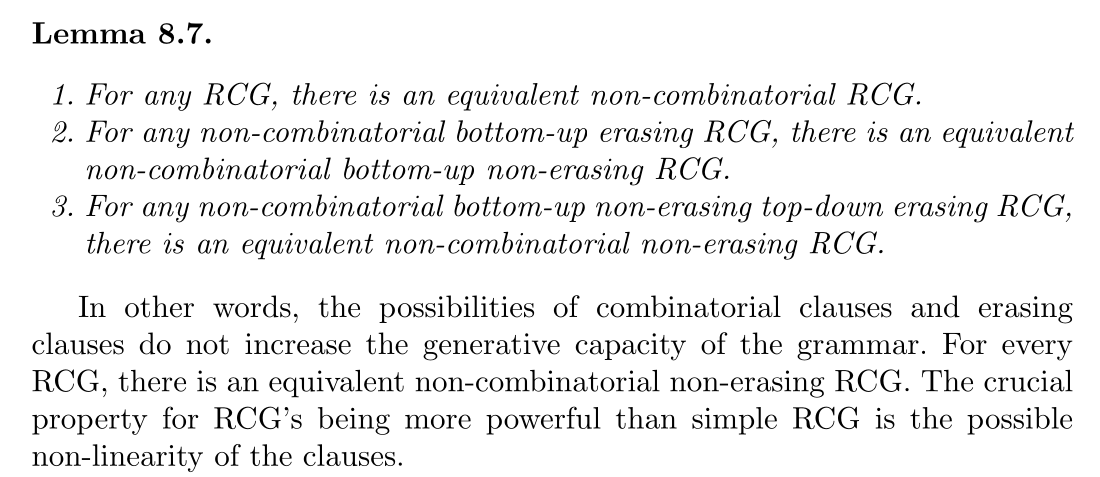
\includegraphics[width=0.88\textwidth]{../media/oponencia-3.png}\\[0.4em]
    {\scriptsize Kallmeyer (2010), \emph{Parsing Beyond Context-Free Grammars}, Lemma 8.7, p.~163.}
  \end{center}
\end{frame}

\begin{frame}{Oponencia --- pregunta 3 (respuesta)}
  \textbf{¿Cuánto cuesta la transformación?}

  Boullier la da en tres pasos locales (Propiedades 1--3):
  \begin{itemize}
    \item<2-> No combinatoria: cada cláusula combinatoria $\to$ tres cláusulas.
    \item<3-> No borrante (lado derecho, bottom-up): el predicado izquierdo gana un argumento con esa variable.
    \item<4-> No borrante (lado izquierdo, top-down): se añade un predicado $\mathrm{Any}$ que acepta cualquier cadena.
  \end{itemize}

  \vspace{0.3em}
  {\scriptsize Boullier (1998), \emph{A Proposal for a Natural Language Processing Syntactic Backbone}, Properties 1--3, pp.~11--12.}
\end{frame}

\begin{frame}{Oponencia --- pregunta 3 (respuesta)}
  \textbf{Ejemplo 1: no combinatoria}

  Cláusula combinatoria ($XY$ no es una variable suelta):
  \[ A(X,Y) \to B(XY) \]

  \pause
  Se reemplaza por tres cláusulas con predicados nuevos $c, c'$:
  \begin{align*}
    A(W, X, Y) &\to c(W, X, Y, W) \\
    c(W, X, Y, U\,Z\,V) &\to c'(X, Y, Z)\; B(W, Z) \\
    c'(X, Y, XY) &\to \varepsilon
  \end{align*}

  \pause
  \azul{$c'(X,Y,XY)$ usa la no linealidad para pegar las piezas.}
\end{frame}

\begin{frame}{Oponencia --- pregunta 3 (respuesta)}
  \textbf{Ejemplo 2: borrado (lado derecho, bottom-up)}

  $Y$ aparece solo a la derecha:
  \[ A(X) \to B(X, Y) \]

  \pause
  Se le da a $A$ un argumento nuevo con $Y$:
  \[ A(Y, X) \to B(X, Y) \]

  \pause
  \azul{Ahora $Y$ está en ambos lados.}
\end{frame}

\begin{frame}{Oponencia --- pregunta 3 (respuesta)}
  \textbf{Ejemplo 3: borrado (lado izquierdo, top-down)}

  Cláusula borrante (la $Y$ solo está a la izquierda):
  \[ A(XY) \to B(X) \]

  \pause
  Se reescribe añadiendo $\mathrm{Any}(Y)$:
  \[ A(XY) \to B(X)\,\mathrm{Any}(Y) \]
  \[ \mathrm{Any}(aX)\to\mathrm{Any}(X), \qquad \mathrm{Any}(\varepsilon)\to\varepsilon \]
  \begin{center}{\small \destacar{($a$ es un terminal cualquiera)}}\end{center}

  \pause
  $\mathrm{Any}$ acepta cualquier cadena: $Y$ se consume sin restringir nada, mismo lenguaje.

  \pause
  \azul{Es el mismo $\mathrm{Any}$ que, al intersectar con $A$, se vuelve $\mathrm{Reach}$ (pregunta 2).}
\end{frame}

\begin{frame}{Oponencia --- pregunta 3 (respuesta)}
  \textbf{Por qué es polinomial}
  \begin{itemize}
    \item<1-> Propiedad 1: cada cláusula combinatoria da a lo sumo 3 (factor constante).
    \item<2-> Propiedad 2: sube la aridad, no el número de cláusulas.
    \item<3-> Propiedad 3: añade $\mathrm{Any}(Y)$ y un bloque fijo de $O(|T|)$ cláusulas.
    \item<4-> $G_{\mathrm{cons}}$ ya es no borrante y no combinatoria.
  \end{itemize}
\end{frame}

\begin{frame}{Oponencia --- pregunta 3 (respuesta)}
  \textbf{Por qué la igualdad de rangos basta}
  \begin{itemize}
    \item<1-> Una variable repetida es la misma pieza de $w$ en varios predicados.
    \item<2-> En el recorrido real, esa pieza se atraviesa una vez: un solo par de estados.
    \item<3-> \destacar{La condición obliga a que todas sus ocurrencias lleven ese par.}
    \item<4-> Sin ella, los índices describirían un recorrido falso, y $G'$ aceptaría cadenas fuera de la intersección.
  \end{itemize}
\end{frame}

\end{document}
